\documentclass[20pt,twocolumn]{article}
\usepackage{geometry}
\geometry{verbose,headsep=3cm,tmargin=2.5cm,bmargin=2.5cm,lmargin=2.0cm,rmargin=2.0cm}
\usepackage{graphicx}
\usepackage{xcolor}
\usepackage[font=small]{caption}
\usepackage{cleveref}
\usepackage{amsmath,amssymb,latexsym}
\usepackage{marvosym}
\usepackage{url}
\usepackage{lipsum}
\usepackage{bm}
\usepackage{float}
\usepackage[english]{babel}
\usepackage{hyperref}
\usepackage{epsf}
\usepackage{float}
\usepackage{mathpazo}
\usepackage{pifont}
\usepackage{wrapfig}
\usepackage{multicol}
\usepackage{enumitem}
\usepackage{xcolor}
\usepackage{framed}
\usepackage[utf8]{inputenc}
\graphicspath{{DWGs/}}

\newcommand{\highlight}[1]{%
  \colorbox{orange!50}{$\displaystyle#1$}}

\begin{document}

\twocolumn[{
\begin{@twocolumnfalse}


  \begin{center}

    \vskip-3em

    \hfill
    \textbf{Bruxelles, November 2018}

    \rule{\textwidth}{0.5pt}
    \vskip2ex

    {\Large\textbf{Condensed Combustion Notes}}
  
    \vspace{2ex}

      \vspace{1ex}
   
	\texttt{https://camillejr.github.io/science-docs/}
          
  \noindent%
    
\vskip1ex

\rule{\textwidth}{0.5pt}

  \end{center}
  
\vspace{8mm}

\end{@twocolumnfalse}
}]

\vspace{10mm}

\setlength{\parindent}{0cm}

\section*{Acknowledgements}

This document was produced during my PhD at Université libre de Bruxelles.

\section{Basic concepts}


\subsection{Species}

\textit{Species} is a general name for any chemical compound that can take role in chemical reaction. In the context of combustion the most encountered species are for instance: CO2, CO, H2O, O2, N2, etc.

\subsection{Species mass fraction}

A species mass fraction is a ratio between mass $m_i$ of a particular $i$-th species in the mixture and the total mass of the mixture $m_{TOT}$:

\begin{equation}
Y_i = \frac{m_i}{m_{TOT}}
\end{equation}

\subsection{Species mole fraction}

A species molar fraction is the ratio between number of moles $N_i$ of a particular $i$-th species in the mixture and the total number of moles of the mixture $N_{TOT}$:

\begin{equation}
\chi_i = \frac{N_i}{N_{TOT}}
\end{equation}

\subsection{Mass-basis and molar-basis quantities}

In combustion, we encounter both \textit{mass-basis} and \textit{molar-basis} quantities. According to [\ref{bib:pitsch}], the mass-basis is useful because mass is conserved and molar-basis is useful because chemical reactions are written per-molar basis.



\subsection{Air-to-fuel ratio}

Air-to-fuel ratio is the ratio between mass of air $m_{air}$ and mass of fuel $m_{fuel}$ in the mixture.

The stoichiometric air-to-fuel ratio:

\begin{equation}
AF_{st} = \Big( \frac{m_{air}}{m_{fuel}} \Big)_{st}
\end{equation}

And a general air-to-fuel ratio for any mixture:

\begin{equation}
AF = \frac{m_{air}}{m_{fuel}}
\end{equation}

\subsection{Equivalence ratio}

The equivalence ratio is the ratio between stoichiometric air-to-fuel ratio and an actual air-to-fuel ratio:

\begin{equation}
\phi = \frac{AF_{st}}{AF}
\end{equation}

When the real mixture has excess air (it is a \textbf{lean} mixture), $\phi < 1$. For \textbf{rich} mixtures $\phi > 1$.





\subsection{Mixture fraction}

In general, when we create an unburnt mixture from fuel and oxidizer streams, the \textit{fuel stream} is composed of fuel and other fuel-impurities and the \textit{oxidizer stream} is composed of oxidizer and other oxidizer-impurities. The mass of the total fuel stream is $m_1$ and the mass of the total oxidizer stream is $m_2$.

The mixture fraction is the ratio between mass of the fuel stream to the total mass of the unburnt mixture:

\begin{equation}
Z = \frac{m_1}{m_{u, TOT}} = \frac{m_1}{m_1 + m_2}
\end{equation}

\begin{figure}[H]
\centering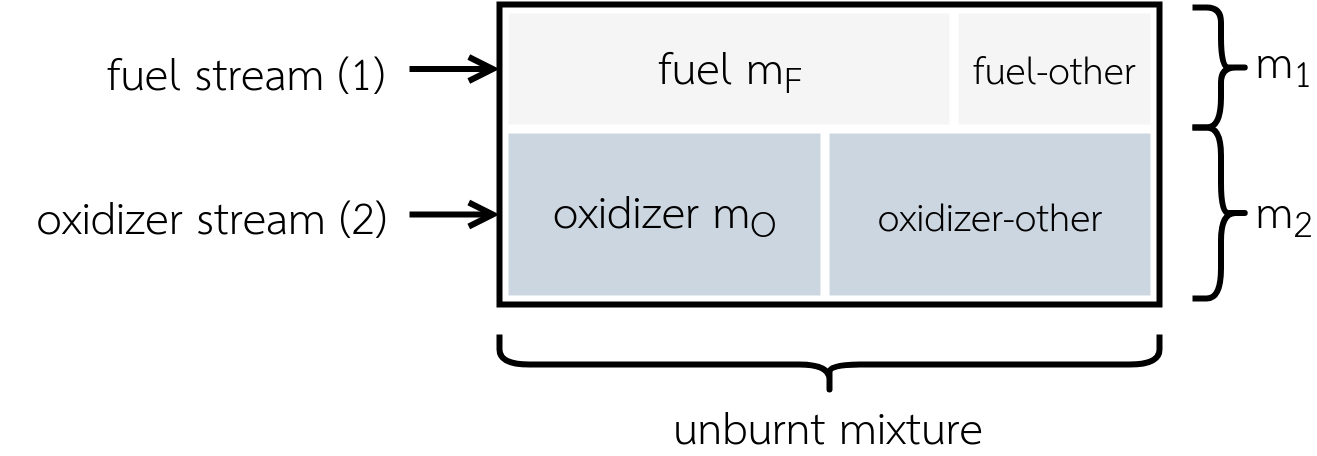
\includegraphics[width=8cm]{mixture-fraction.png}
\caption{Mixture fraction notion.}			
\label{fig:mixture-fraction}
\end{figure}


We may also define the mass fraction of fuel in the unburnt mixture:

\begin{equation}
Y_{u, F} = \frac{m_F}{m_{u, TOT}} = \frac{m_F}{m_1 + m_2}
\end{equation}

and mass fraction of fuel in the fuel stream:

\begin{equation}
Y_{1, F} = \frac{m_F}{m_1}
\end{equation}

These two quantities are clearly related to each other via the mixture fraction:

\begin{equation}
Y_{u, F} = \frac{m_F}{m_1 + m_2} = \frac{m_F}{m_1} \frac{m_1}{m_1 + m_2} = Y_{1, F} Z
\end{equation}

Similar reasoning can be done for the oxidizer in the oxidizer stream.



\subsection{Adiabatic flame temperature}

Adiabatic flame temperature is the temperature of combustion products if the combustion happens without heat exchange with the surroundings. It thus has the meaning of maximum possibly achievable temperature for a given combustion.

\subsubsection{Constant pressure AdFT}



\subsubsection{Constant volume AdFT}











\section{Energy considerations}







\section{Transfer equations}




\section{Chemical reactors}







\appendix

\section{APP1} \label{app:A}

\section{APP2} \label{app:B}

\thebibliography{}

\bibitem{Turns} S. R. Turns, \textit{An Introduction to Combustion: Concepts and Applications}, Second Edition, 2000 \label{bib:turns}

\bibitem{Pitsch} H. Pitsch, \textit{Combustion Theory and Applications in CFD}, Lecture Series \label{bib:pitsch}


 \label{bib:pope}


\end{document}
